% --------------------------------------------------------------------------- %
% Poster for the ECCS 2011 Conference about Elementary Dynamic Networks.      %
% --------------------------------------------------------------------------- %
% Created with Brian Amberg's LaTeX Poster Template. Please refer for the     %
% attached README.md file for the details how to compile with `pdflatex`.     %
% --------------------------------------------------------------------------- %
% $LastChangedDate:: 2011-09-11 10:57:12 +0200 (V, 11 szept. 2011)          $ %
% $LastChangedRevision:: 128                                                $ %
% $LastChangedBy:: rlegendi                                                 $ %
% $Id:: poster.tex 128 2011-09-11 08:57:12Z rlegendi                        $ %
% --------------------------------------------------------------------------- %
\documentclass[a0paper,portrait]{baposter}

\usepackage{relsize}		% For \smaller
\usepackage{url}			% For \url
\usepackage{epstopdf}	% Included EPS files automatically converted to PDF to include with pdflatex
\usepackage{moresize}
\usepackage{multicol}

%%% Global Settings %%%%%%%%%%%%%%%%%%%%%%%%%%%%%%%%%%%%%%%%%%%%%%%%%%%%%%%%%%%

\graphicspath{{pix/}}	% Root directory of the pictures 
\tracingstats=2			% Enabled LaTeX logging with conditionals

%%% Color Definitions %%%%%%%%%%%%%%%%%%%%%%%%%%%%%%%%%%%%%%%%%%%%%%%%%%%%%%%%%

\definecolor{bordercol}{RGB}{40,40,40}
\definecolor{headercol1}{HTML}{DEEEB2}
\definecolor{headercol2}{RGB}{80,80,80}
\definecolor{headerfontcol}{RGB}{0,0,0}
\definecolor{boxcolor}{HTML}{ffffff}

%\definecolor{orange}{HTML}{FF7F00}

%%%%%%%%%%%%%%%%%%%%%%%%%%%%%%%%%%%%%%%%%%%%%%%%%%%%%%%%%%%%%%%%%%%%%%%%%%%%%%%%
%%% Utility functions %%%%%%%%%%%%%%%%%%%%%%%%%%%%%%%%%%%%%%%%%%%%%%%%%%%%%%%%%%

%%% Save space in lists. Use this after the opening of the list %%%%%%%%%%%%%%%%
\newcommand{\compresslist}{
	\setlength{\itemsep}{1pt}
	\setlength{\parskip}{0pt}
	\setlength{\parsep}{0pt}
}

%%%%%%%%%%%%%%%%%%%%%%%%%%%%%%%%%%%%%%%%%%%%%%%%%%%%%%%%%%%%%%%%%%%%%%%%%%%%%%%
%%% Document Start %%%%%%%%%%%%%%%%%%%%%%%%%%%%%%%%%%%%%%%%%%%%%%%%%%%%%%%%%%%%
%%%%%%%%%%%%%%%%%%%%%%%%%%%%%%%%%%%%%%%%%%%%%%%%%%%%%%%%%%%%%%%%%%%%%%%%%%%%%%%

\begin{document}
\typeout{Poster rendering started}

%%% Setting Background Image %%%%%%%%%%%%%%%%%%%%%%%%%%%%%%%%%%%%%%%%%%%%%%%%%%
\background{
%	\begin{tikzpicture}[remember picture,overlay]%
%	\draw (current page.north west)+(-2em,2em) node[anchor=north west]
%	{\includegraphics[height=1.1\textheight]{background}};
%	\end{tikzpicture}
}

%%% General Poster Settings %%%%%%%%%%%%%%%%%%%%%%%%%%%%%%%%%%%%%%%%%%%%%%%%%%%
%%%%%% Eye Catcher, Title, Authors and University Images %%%%%%%%%%%%%%%%%%%%%%
\begin{poster}{
	grid=false,
	% Option is left on true though the eyecatcher is not used. The reason is
	% that we have a bit nicer looking title and author formatting in the headercol
	% this way
	%eyecatcher=false, 
	borderColor=bordercol,
	headerColorOne=headercol1,
	headerColorTwo=headercol2,
	headerFontColor=headerfontcol,
	% Only simple background color used, no shading, so boxColorTwo isn't necessary
	boxColorOne=boxcolor,
	headershade=plain,
	boxColorTwo=green,
	headershape=roundedright,
	headerfont=\Large\sf\bf,
	textborder=rectangle,
	background=user,
%  	boxshade=shade-lr,
  	headerborder=closed
}
%%% Eye Cacther %%%%%%%%%%%%%%%%%%%%%%%%%%%%%%%%%%%%%%%%%%%%%%%%%%%%%%%%%%%%%%%
{
	Eye Catcher, empty if option eyecatcher=false - unused
}
%%% Title %%%%%%%%%%%%%%%%%%%%%%%%%%%%%%%%%%%%%%%%%%%%%%%%%%%%%%%%%%%%%%%%%%%%%
{\sf\bf
	A Topography of Climate Change Research
}
%%% Authors %%%%%%%%%%%%%%%%%%%%%%%%%%%%%%%%%%%%%%%%%%%%%%%%%%%%%%%%%%%%%%%%%%%
{
	\vspace{0.4em} \url{https://dx.doi.org/10.1038/s41558-019-0684-5}\\
	Max Callaghan\\
	{\smaller callaghan@mcc-berlin.net}
}
%%% Logo %%%%%%%%%%%%%%%%%%%%%%%%%%%%%%%%%%%%%%%%%%%%%%%%%%%%%%%%%%%%%%%%%%%%%%
{
% The logos are compressed a bit into a simple box to make them smaller on the result
\setlength\fboxsep{0pt}
\setlength\fboxrule{0.5pt}
	\fbox{
		\begin{minipage}{14em}
			\begin{minipage}{7em}
				\centering
			\vspace*{0.005\textheight}
			\includegraphics[width=6.5em]{../pres/MCC_Logo_RZ_rgb.jpg}
			\\
			\vspace*{0.005\textheight}
			\includegraphics[width=6.5em]{../pres/University_of_Leeds_Logo.png}
			\vspace*{0.005\textheight}
			\end{minipage}
			\begin{minipage}{7em}
				\centering
			\includegraphics[width=6.5em]{../pres/logo_hbs.jpg}
			\end{minipage}
		\end{minipage}
	}
}



\headerbox{Problem}{name=problem,column=0,row=0}{

\includegraphics[width=\linewidth]{../plots/literature_size/pubs_time_wgb_lp.pdf}

Massive growth of literature on climate change challenges IPCC \cite{Minx2017l}

}

\headerbox{Proportionality}{name=definitions,column=0,below=problem}{
\begin{center}
	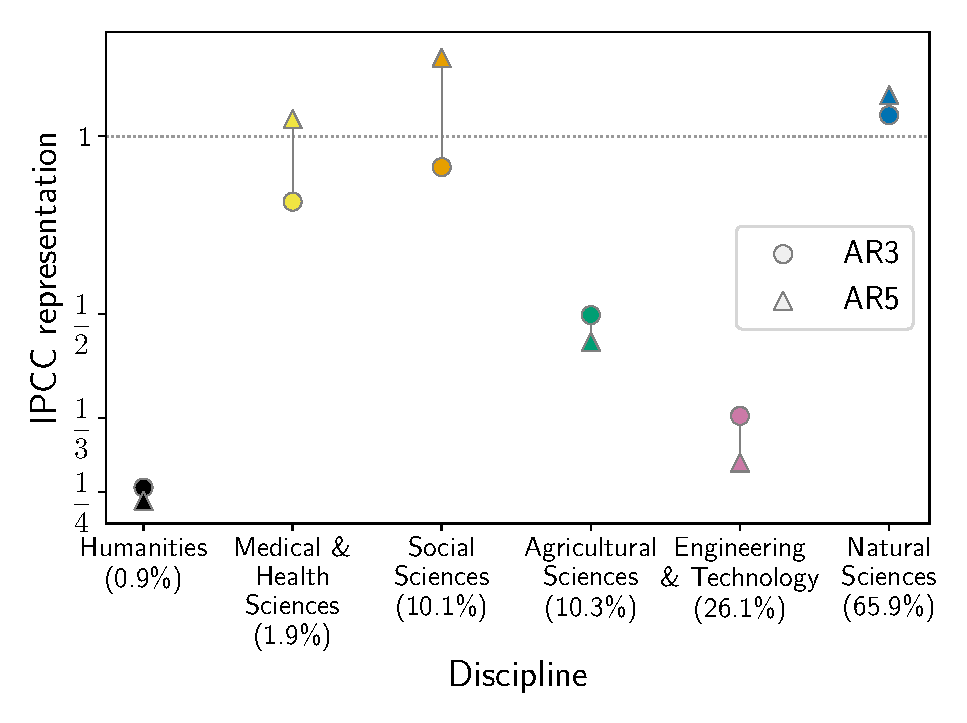
\includegraphics[width=0.98\linewidth]{../plots_pub/ipcc_rep_oecds_simplified_lp.pdf}
	
\end{center}
\vspace{-1.4em} 
Contrary to suggestions/previously \cite{Victor2015, Bjurstroem2011}, the social sciences are over-represented in IPCC reports, engineering/agricultural sciences are under-represented
}

\headerbox{Supply/Demand of Solutions}{name=models,column=0,below=definitions}{

\begin{center}
	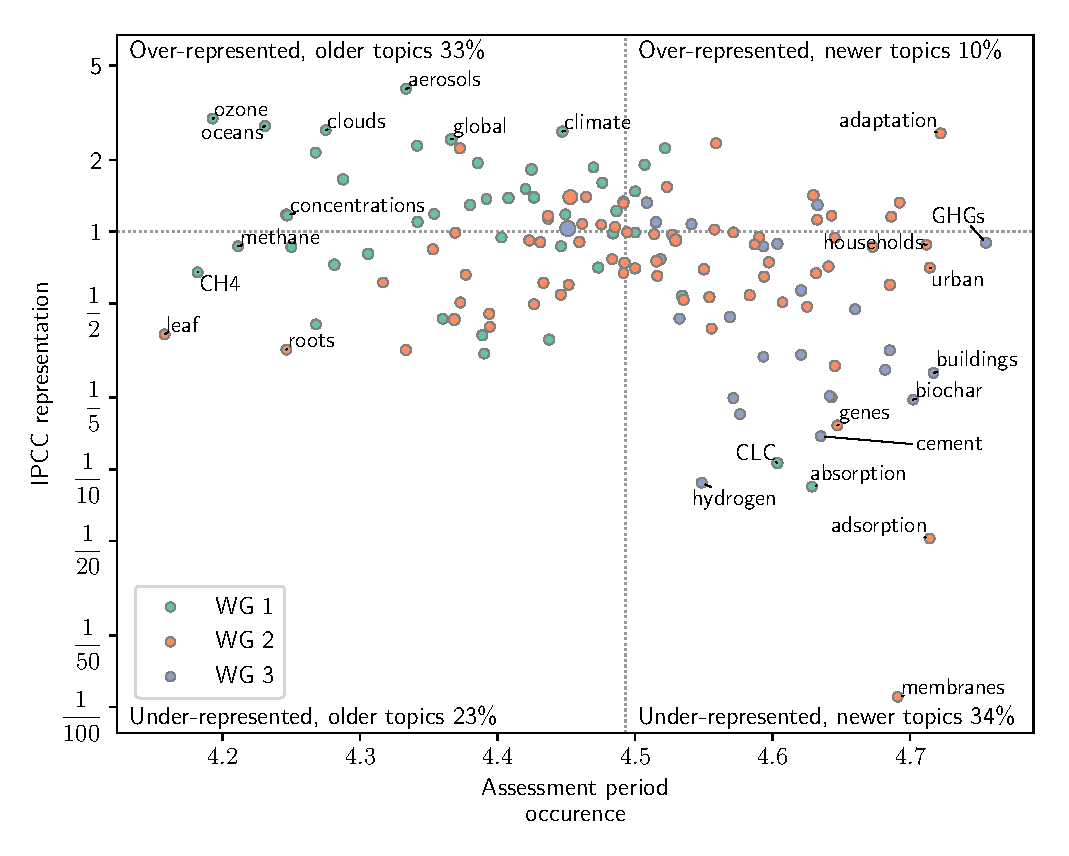
\includegraphics[width=0.98\linewidth]{../plots_pub/rep_time_lp.pdf}
\end{center}

\vspace{-1.4em}

Physical science topics are well represented and have been around longer. Solution-oriented topics, particularly in WGIII are newer and under-represented.

}

\headerbox{References}{name=references,column=0,below=models}{
\tiny												% Make the whole text smaller
\vspace{-0.4em} 										% Save some space at the beginning
\bibliographystyle{plain}							% Use plain style
\renewcommand{\section}[2]{\vskip 0.05em}		% Omit "References" title
\smaller
\bibliography{../Mendeley}
}

\headerbox{Acknowledgements}{name=acknowledgements,column=0,below=references, above=bottom}{
\smaller						% Make the whole text smaller
%\vspace{-0.4em}			% Save some space at the beginning
This research is funded by a PhD scholarship from the Heinrich Böll Stiftung
} 

\headerbox{New Concepts}{name=concepts,span=2,column=1,row=0}{
	{\scriptsize\resizebox{\textwidth}{!}{
	\input{../tables/growth_table.tex}}}

	A simple analysis of the words in the documents about climate change shows us that not only are there more articles, they discuss \textbf{new concepts}. The \textbf{topic model} below \cite{Lee1999} mobilises large patterns of words in documents to make broad conceptual developments and differences comprehensible.
}

\headerbox{A Topographic Map of 400,000 Climate Change Articles}{name=density,span=2,column=1,below=concepts}{

\begin{minipage}{0.74\linewidth}
	\begin{center}
	\includegraphics[width=1\linewidth]{../plots_pub/all_topic_words_oecds.png}
	\end{center}
\end{minipage}
\begin{minipage}{0.24\linewidth}
	Using T-SNE \cite{vandermaaten2008}, we can project each document into a 2D space such that documents with similar 100-dimensional topic vectors are close together.
	
	\medskip
	
	 Documents similar in topic tend to be from similar disciplines, with some cross-disciplinary work around the energy system, or on soils.
	 
	 \medskip
	 
	 The majority of topics are from the natural sciences
\end{minipage}
%\begin{minipage}{0.3\linewidth}
%\end{minpage}

}

\headerbox{Evolution }%Interdisciplinarity}
{name=degreeDistribution,span=1,column=1,below=density,above=bottom}{
	
\begin{center}
	\includegraphics[width=0.98\linewidth]{../plots_pub/topic_evolution_4.png}
\end{center}

Solutions topics have grown fast in recent assessment reports, as have topics on impacts and vulnerability. New WGII topics are better covered by IPCC reports. We can also witness the emergence of new topics such as coral bleaching.
	
}

\headerbox{Social Science \& Solutions}
{name=socSciSol,span=1,column=2,below=density}{
	\begin{center}
		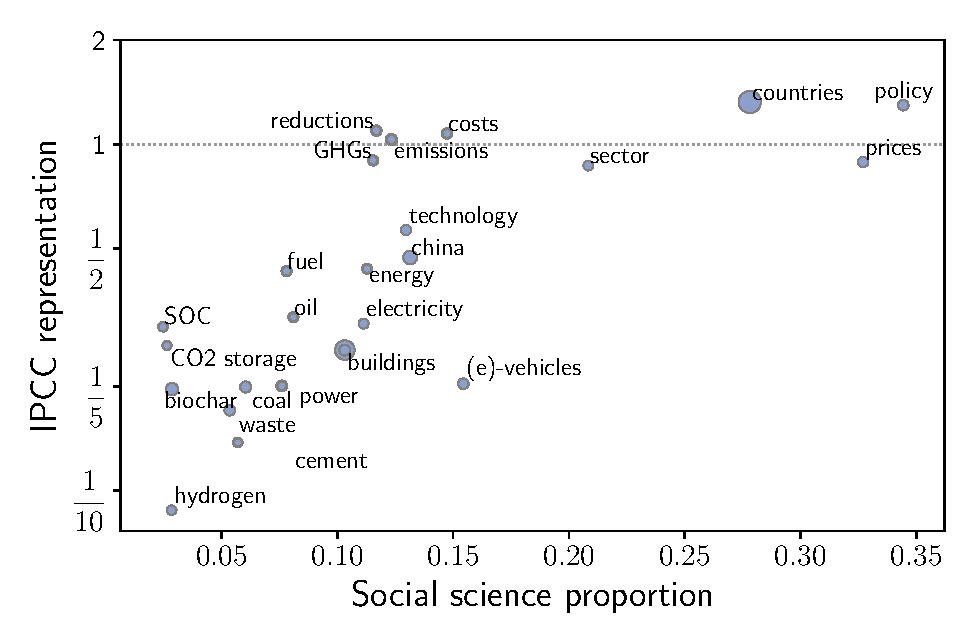
\includegraphics[width=0.98\linewidth]{../plots/run_1861_wg3_socsci_lp.pdf}
	\end{center}
	\vspace{-1.4em}
Those WGIII topics with a higher share of social science documents are better-represented in IPCC. Either the IPCC must engage with the social science literature, or the social sciences must cover solutions-topics.
}

\headerbox{Further work}
{name=further,span=1,column=2,below=socSciSol,above=bottom}{

Computer-assisted systematic map of climate impacts.

Robust Statistical Stopping Criteria for Automated
Screening in Systematic Reviews





}


\end{poster}
\end{document}
